\begin{figure}[t]
\centering
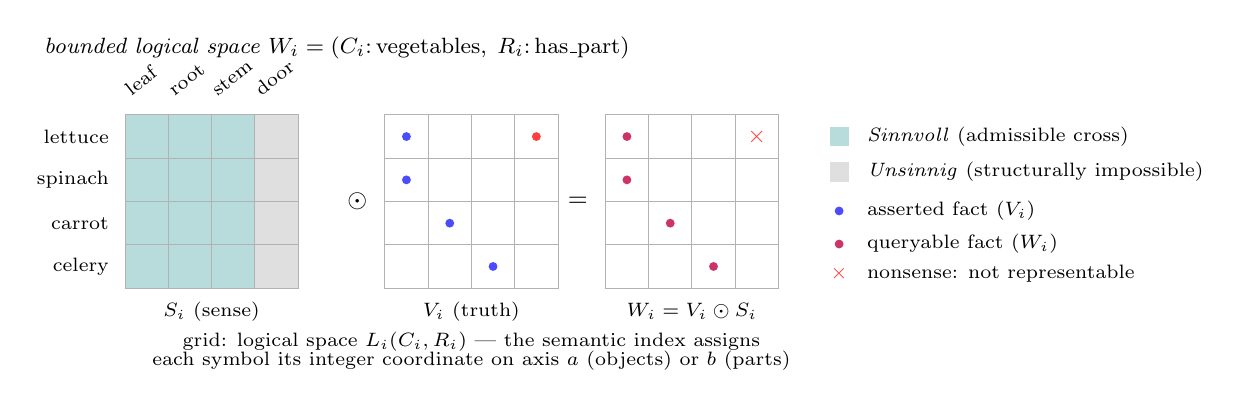
\begin{tikzpicture}[font=\small]
  \node[font=\footnotesize\itshape, anchor=west] at (-1.15,-0.75) {bounded logical space $W_i=(C_i\colon \mathrm{vegetables},\; R_i\colon \mathrm{has\_part})$};
  % S_i
  \foreach \r in {0,1,2,3} \foreach \c in {0,1,2} \fill[teal!28] ({0.55*\c},{-1.6-0.55*\r}) rectangle ++(0.55,-0.55);
  \foreach \r in {0,1,2,3} \fill[gray!25] ({0.55*3},{-1.6-0.55*\r}) rectangle ++(0.55,-0.55);
  \foreach \r in {0,1,2,3} \foreach \c in {0,1,2,3} \draw[gray!60, line width=0.3pt] ({0.55*\c},{-1.6-0.55*\r}) rectangle ++(0.55,-0.55);
  \foreach \r/\n in {0/lettuce, 1/spinach, 2/carrot, 3/celery} \node[font=\scriptsize, anchor=east] at (-0.08,{-1.875-0.55*\r}) {\n};
  \foreach \c/\n in {0/leaf, 1/root, 2/stem, 3/door} \node[font=\scriptsize, rotate=38, anchor=south west] at ({0.06+0.55*\c},-1.54) {\n};
  \node[font=\scriptsize] at (1.1,-4.1) {$S_i$ (sense)};
  % V_i
  \node at (2.95,-2.7) {$\odot$};
  \foreach \r in {0,1,2,3} \foreach \c in {0,1,2,3} \draw[gray!60, line width=0.3pt] ({3.3+0.55*\c},{-1.6-0.55*\r}) rectangle ++(0.55,-0.55);
  \fill[blue!70] (3.575,-1.875) circle (1.6pt);
  \fill[blue!70] (3.575,-2.425) circle (1.6pt);
  \fill[blue!70] (4.125,-2.975) circle (1.6pt);
  \fill[blue!70] (4.675,-3.525) circle (1.6pt);
  \fill[red!75]  (5.225,-1.875) circle (1.6pt);
  \node[font=\scriptsize] at (4.4,-4.1) {$V_i$ (truth)};
  % W_i
  \node at (5.75,-2.7) {$=$};
  \foreach \r in {0,1,2,3} \foreach \c in {0,1,2,3} \draw[gray!60, line width=0.3pt] ({6.1+0.55*\c},{-1.6-0.55*\r}) rectangle ++(0.55,-0.55);
  \fill[purple!80] (6.375,-1.875) circle (1.6pt);
  \fill[purple!80] (6.375,-2.425) circle (1.6pt);
  \fill[purple!80] (6.925,-2.975) circle (1.6pt);
  \fill[purple!80] (7.475,-3.525) circle (1.6pt);
  \node[red!75, font=\footnotesize] at (8.025,-1.875) {$\times$};
  \node[font=\scriptsize] at (7.2,-4.1) {$W_i = V_i \odot S_i$};
  \node[font=\scriptsize, align=center] at (4.4,-4.6) {grid: logical space $L_i(C_i,R_i)$ --- the semantic index assigns\\[-1pt]{each symbol its integer coordinate on axis $a$ (objects) or $b$ (parts)}};
  % legend
  \fill[teal!28] (8.95,-1.75) rectangle ++(0.25,-0.25); \node[font=\scriptsize, anchor=west] at (9.3,-1.875) {\emph{Sinnvoll} (admissible cross)};
  \fill[gray!25] (8.95,-2.2) rectangle ++(0.25,-0.25); \node[font=\scriptsize, anchor=west] at (9.3,-2.325) {\emph{Unsinnig} (structurally impossible)};
  \fill[blue!70] (9.07,-2.82) circle (1.6pt); \node[font=\scriptsize, anchor=west] at (9.3,-2.82) {asserted fact ($V_i$)};
  \fill[purple!80] (9.07,-3.24) circle (1.6pt); \node[font=\scriptsize, anchor=west] at (9.3,-3.24) {queryable fact ($W_i$)};
  \node[red!75, font=\scriptsize] at (9.07,-3.62) {$\times$}; \node[font=\scriptsize, anchor=west] at (9.3,-3.62) {nonsense: not representable};
\end{tikzpicture}
\caption{The discrete primitives proposed in this work, inside one bounded logical space $W_i=(C_i{:}\,\mathrm{vegetables},R_i{:}\,\mathrm{has\_part})$ (categories match the worked example of \S3). The shared grid is the logical space $L_i(C_i,R_i)$: the semantic index that assigns every symbol an integer coordinate on axis $a$ (objects) or axis $b$ (parts). The sense mask $S_i$ (left) separates meaningful crosses (\emph{Sinnvoll}, teal) from structural absurdities (\emph{Unsinnig}, grey: vegetables have no \emph{door}); the truth layer $V_i$ (center) stores asserted facts (dots). Only the product $W_i=V_i\odot S_i$ (right) is queryable: a fact outside the mask---$(\mathrm{part}\ \mathrm{lettuce}\ \mathrm{door})$---is not false but structurally impossible to represent ($\times$).}
\label{fig:layers}
\end{figure}
